% !TEX spellcheck = en-US
\documentclass[aps,prl,twocolumn,amsmath,amssymb,superscriptaddress,nobibnotes]{revtex4}%
\usepackage{graphicx}
\usepackage{dcolumn}
\usepackage{bm}
\usepackage{color}
\usepackage{amsmath}
\usepackage{epstopdf}
%\usepackage{caption}
%\usepackage{subcaption}
\usepackage{fancybox}
\usepackage{amsfonts}
\usepackage{amssymb}%
\usepackage[toc,page]{appendix}
%\usepackage[backend=bibtex,natbib=true,sorting=none]{biblatex}
\setcounter{MaxMatrixCols}{30}


\renewcommand{\cite}[1]{{[}\onlinecite{#1}{]}}

\newcommand{\s}{\sum\limits}
\newcommand{\p}{\prod\limits}
\newcommand{\pa}{\partial}
\newcommand{\il}{\int\limits}
\newcommand{\be}{\begin{equation}}
\newcommand{\e}{\end{equation}}
\newcommand{\beml}{\begin{subequations}}
\newcommand{\eml}{\end{subequations}}
\newcommand{\beq}{\begin{eqnarray}}
\newcommand{\eq}{\end{eqnarray}}
\newcommand{\ba}{\begin{array}}
\newcommand{\ea}{\end{array}}
\newcommand{\bpm}{\begin{pmatrix}}
\newcommand{\epm}{\end{pmatrix}}
\newcommand{\bc}{\begin{cases}}
\newcommand{\ec}{\end{cases}}
\newcommand{\lt}{\left}
\newcommand{\rt}{\right}
\newcommand{\n}{\nonumber}
\newcommand{\la}{\langle}
\newcommand{\ra}{\rangle}
\newcommand{\ep}{\varepsilon}
\newcommand{\dd}{\displaystyle}
\newcommand{\bs}{\boldsymbol}
\newcommand{\h}{^\dagger}
\newcommand{\ph}{^{\phantom{\dagger}}}
\newcommand{\one}{\openone}
\newcommand{\ut}{\underaccent{\tilde}}
\newcommand{\ul}{\underaccent{\bar}}
\newcommand{\up}{\uparrow}
\newcommand{\dn}{\downarrow}
\DeclareMathOperator{\var}{var}
\DeclareMathOperator{\tr}{Tr}
\DeclareMathOperator{\diag}{diag}
\DeclareMathOperator{\im}{Im}
\DeclareMathOperator{\re}{Re}
\DeclareMathOperator{\ctg}{cotan}
\DeclareMathOperator{\arcsh}{arcsinh}
\DeclareMathOperator{\csch}{csch}
\DeclareMathOperator{\rot}{rot}

\newcommand{\AQ}[1]{\textbf{\textcolor{red}{{#1}}}}

\begin{document}
\title{Ultrafast manipulation of Heisenberg exchange and Dzyaloshinskii–-Moriya interactions in antiferromagnetic insulators}


\begin{abstract}
This is the abstract.
\end{abstract}

\date{\today}
\maketitle

\begin{section}{Model and calculations}

The first model to describe topological insulators was introduced by Kane and Mele \cite{Kane2005} to describe quantum spin Hall effect in graphene. In a honeycomb lattice time reversal symmetry and inversion symmetry allow only next-nearest neighbor spin orbit coupling, which is known as intrinsic spin orbit coupling. In these circumstances the system can be modeled by the Kane-Mele-Hubbard which we write as a sum of a kinetic term, an interaction term and a SOI term:

\begin{equation}
\label{MKMH}
\hat{H}^0 = \hat{\mathcal{H}}_t + \hat{\mathcal{H}}_{\text{SOI}} + \hat{\mathcal{H}}_{\text{int}}
\end{equation}
Where:
\begin{align}
&\hat{\mathcal{H}}_t = - \sum_{\langle i,j \rangle, \sigma} t_1\hat{c}_{i \sigma}^\dagger \hat{c}_{j \sigma} - \sum_{\langle \langle i,j \rangle \rangle, \sigma} t_2\hat{c}_{i \sigma}^\dagger \hat{c}_{j \sigma} \\
&\hat{\mathcal{H}}_{\text{SOI}} = \sum_{\langle \langle i,j \rangle \rangle, \sigma} i\Delta\nu_{ij}\sigma^z_{\sigma, \sigma}\hat{c}_{i \sigma}^\dagger \hat{c}_{j \sigma} \\
&\hat{\mathcal{H}}_{\text{int}} = \text{U}_{00}\sum_{i=1}^M \hat{n}_{i\uparrow}\hat{n}_{i\downarrow} + \frac{1}{2}\sum_{\langle i,j \rangle, \sigma \sigma'} \text{U}_{ij}\hat{n}_{i\sigma}\hat{n}_{j\sigma'}
\end{align}

Where $\hat{c}_{i \sigma}^\dagger$ ($ \hat{c}_{i \sigma}$) creates (anihilates) an electron at site $i$ in spin state $\sigma$, $\text{U}_{00}$ and $\text{U}_{ij}$ are the on-site and NN Coulomb interactions. $t_1$, $t_2$ are the hopping amplitudes originating from both kinetic hopping. $\Delta$ is the intrinsic spin orbit coupling constant. $\nu_{ij}=\pm 1$ depending on whether the electron traversing from $i$ to $j$ makes a right ($+1$) or a left turn ($-1$). $\sigma^{z}$ is the third Pauli matrix. 
In practice the NN Coulomb interaction can be effectively approximated by a reduced on-site interaction $\text{U} = \text{U}_{00} - \bar{\text{U}}$ where $\bar{\text{U}}$ is an average of the NN Coulomb interacion \cite{Schuler2013}, we therefore can take:
\begin{equation}
\hat{\mathcal{H}}_{\text{int}} \approx \text{U}\sum_{i=1}^M \hat{n}_{i\uparrow}\hat{n}_{i\downarrow}
\end{equation}
With $\text{U} = \text{U}_{00} - \bar{\text{U}}$.

\begin{figure}[t]
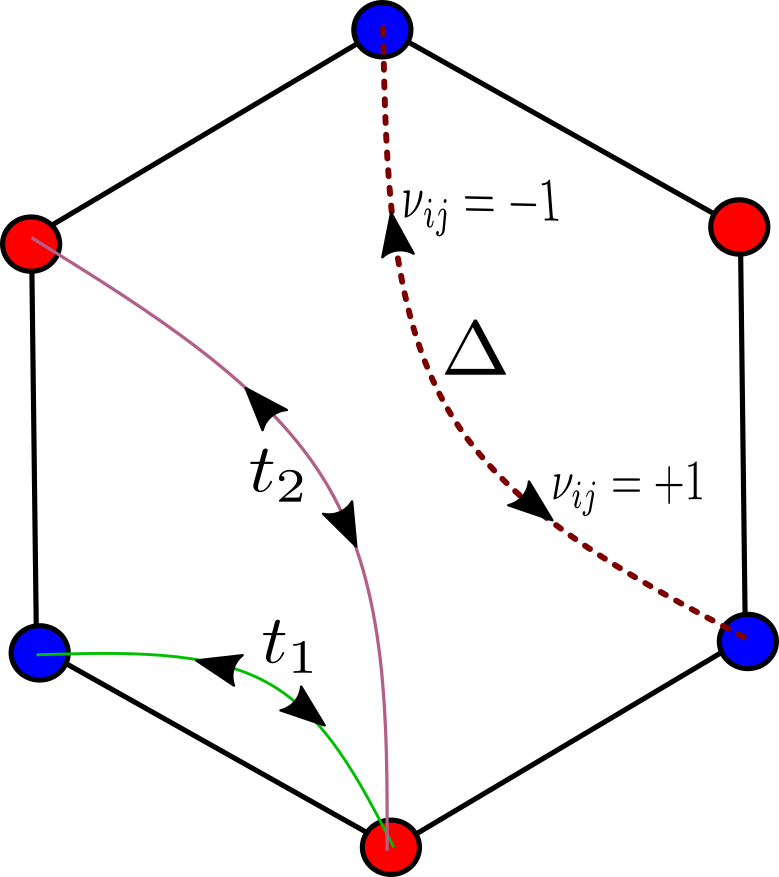
\includegraphics[width=0.6\columnwidth]{../Figures/kmh.png}
\caption{A honycomb cell with NN hopping $t_1$, NNN hopping $t_2$ and intrinsic SOI $\Delta$. $\nu_{ij} = \pm 1$ depending on whether the electron traversing from $i$ to $j$ makes a right ($+1$) or a left turn ($-1$).}
\label{fig1}
\vspace*{-6pt}
\end{figure}
Let us define $\hat{D} = \sum_{i=1}^M \hat{n}_{i\uparrow}\hat{n}_{i\downarrow}$ the doublon number operator so that $\hat{\mathcal{H}}_{\text{int}} \approx \text{U}\hat{D}$ with eigenvalues $d$ and projection operators $\hat{P}_d$. We will assume a half filling system in which the strength of the on-site interaction $\text{U}$ is much larger than the hopping amplitudes. In the strong coupling limit any state with a nonzero number of double occupancies ($d \neq 0$) will have much larger energy than those with $d=0$. We can therfore obtain an effective Hamiltonian acting on the $d=0$ subspace by standard second order perturbation techniques in the hopping terms. We can then obtain the effective spin Hamiltonian by using the relations:
\begin{align}
\hat{c}_{i \sigma}^\dagger \hat{c}_{i \sigma'} &= \delta_{\sigma \sigma'} \frac{1}{2} (n_{i \uparrow} + n_{i \downarrow}) + \bs{S}_i\cdot\bs{\sigma}_{\sigma', \sigma} \label{SpinOperatorInv1}\\ 
\hat{c}_{i \sigma} \hat{c}_{i \sigma'}^\dagger &= \delta_{\sigma \sigma'} \frac{1}{2} (2 - n_{i \uparrow} - n_{i \downarrow}) - \bs{S}_i\cdot\bs{\sigma}_{\sigma, \sigma'} \label{SpinOperatorInv2}
\end{align}
Following this procedure we obtain the following effective spin Hamiltonian:

\begin{align}
\label{MKMHeff0}
&\hat{H}_{\text{eff}} = \sum_{\langle i,j \rangle} J_{1,ij}\bs{S}_i\cdot\bs{S}_j +\n \\
&+ \sum_{\langle \langle i,j \rangle \rangle} \left\{ J_{2,ij}\bs{S}_i\cdot\bs{S}_j + \bs{D}_{2,ij}\cdot \bs{S}_i \times \bs{S}_j + \bs{S}_i \bs{\Gamma}_{ij} \bs{S}_j \right\}
\end{align}

Where:

\begin{align*}
J_{1,ij} &= 2t_1^2 \\
J_{2,ij} &= 2t_2^2 \\
\bs{D}_{2,ij} &= - 4\nu_{ij} t_2 \Delta \hat{e}_z \\
\bs{\Gamma}_{2,ij} &= 2\Delta^2 \text{diag}(-1,-1,1)
\end{align*}

\textit{Introducing laser perturbation}. In the prescence of an laser perturbation we can use the Peirls substitution to include the effect of the field trough the hopping amplitudes. We can write the electric field as $\bs{E}(t) = \frac{1}{2}(\vec{E}e^{-i\omega t}+\vec{E}^*e^{i\omega t})$, $\vec{E} = E_0\hat{e}$ and $\hat{e} = \frac{1}{\sqrt{1+\lambda_{POL}^2}}(\hat{e}_x+i\lambda_{POL}\hat{e}_y)$ is the polarization vector and $\lambda_{POL} = 0, \pm 1$ for plane polarized, right handed and left handed circular polarized field respectively. According to the Peierls rule the hopping amplitudes gain a phase $e^{ie\bs{R}_{ij}\bs{A}(t)}$ where $\bs{R}_{ij} = \bs{R}_i-\bs{R}_j$, $\bs{R}_i$ is the position of site $i$ and $\bs{A}$ is the vector potential $\bs{A}(t) = \frac{1}{2}(\vec{A}e^{-i\omega t} + \vec{A}^* e^{i\omega t})$, with $\vec{A} = \frac{iE_0}{\omega}\hat{e}$.

Let us define:

\begin{equation}
\label{Def_alpha}
e\bs{R}_{ij}\cdot\vec{A} = \alpha_{ij} e^{i \theta_{ij}}
\end{equation}

With $\alpha_{ij} = \pm|e\bs{R}_{ij}\vec{A}|$ in such a way that:

\begin{align}
\alpha_{ij} &= -\alpha_{ji} \label{alphaSym} \\
\theta_{ij} &= \theta_{ji} \label{thetaSym}
\end{align}

and $\theta_{ij} \in \left[0,\pi\right)$. Then we can apply the Jacobi-–Anger expansion to Fourier transform the hopping amplitues:
\begin{equation}
\label{JacobiAnger}
e^{ie\bs{R}_{ij}\cdot\bs{A}(t)} = \sum_m e^{i(\frac{\pi}{2}-\theta_{ij})m} \mathcal{J}_m(\alpha_{ij}) e^{im\omega t} 
\end{equation}
where $\mathcal{J}_m(x)$ is the \textit{m}th Bessel function \cite{Kitamura2017}, modulating the weight of the \textit{m}th Fourier mode of the hopping amplitude. Let $\hat{T}_0$ be the hopping part of the hamiltonian, so that $\hat{H}_0 = \hat{T}_0 + \text{U}\hat{D}$. When an electric field is applied, the hopping amplitudes become time dependent so that $\hat{H}(t) = \hat{T}(t) +  \text{U}\hat{D}$. Using \ref{JacobiAnger} we can write $\hat{T}(t) = \sum_m \hat{T}_m e^{im \omega t}$ where $\hat{T}_m$ is the sum of all the \textit{m}th Fourier mode of the hopping terms. Additionaly we can further decompose the hopping operator into:

\begin{equation}
\hat{T}(t) = \sum_m (\hat{T}_{-1,m}+\hat{T}_{0,m}+\hat{T}_{1,m})e^{im\omega t}
\end{equation}

Where $\hat{T}_{dm}(t)$ changes the doublon number by $d$, for example, if $\hat{P}_d$ is the projection operator into the subspace with doublon number $d$, then $\hat{T}_{dm}(t) = \sum_i \hat{P}_{i+d}\hat{T}_{m}(t)\hat{P}_i$.

In order to derive the form of the effective Hamiltonian let us introduce a time dependent unitary transformation $\hat{U}(t) = e^{-i\hat{S}(t)}$. The transformed Hamiltonian is:

\begin{equation}
\hat{H}'(t) = e^{i\hat{S}(t)} \hat{H}(t) e^{-i\hat{S}(t)} - e^{i\hat{S}(t)} id_t e^{-i\hat{S}(t)}
\label{Htransformed}
\end{equation} 

We perform the unitary transformation perturbatively in the hopping operator, we can formally write $\hat{T}(t) = \eta \hat{T}(t)$, where $\eta$ will play the role of a bookkeeping parameter in the perturbative expansion. We expand $\hat{S}(t) = \sum_\nu \eta^\nu \hat{S}^{(\nu)}(t)$ and $\hat{H}'(t) = \sum_\nu \eta^\nu \hat{H}'^{(\nu)}(t)$. In order for the new Hamiltonian to be periodic we impose the unitary transformation to have the periodicity of the Hamiltonian, so that we can expand $\hat{S}^{(\nu)}(t) = \sum_m e^{im\omega t}\hat{S}^{(\nu)}_m$. Additionally we can impose the transformed Hamiltonian to be block diagonal in the doublon number $d$. With these conditions the unitary transformation can be uniquely determined if we impose that $\hat{S}(t)$ does not contain block-diagonal terms, i.e. we can write:
\begin{equation}
\hat{S}^{(\nu)}(t) = \sum_{d \neq 0} \sum_m \eta^\nu \hat{S}^{(\nu)}_{d,m} e^{im\omega t}
\end{equation}
where $\hat{S}^{(\nu)}_{d,m}$ changes the double occupancy number by $d$. From here the procedure is simple but lenghty, we expand \ref{Htransformed} in power series of $\eta$ and determine $\hat{S}^{(\nu)}(t)$ iteratively in $\nu$ so that $\hat{H}'^{(\nu)}(t)$ is diagonal in the doublon number. Up to second order we obtain:
\begin{align}
&\hat{H}'(t) \approx \text{U}\hat{D} - \sum_m \hat{T}_{0,m}(t)e^{im\omega t} + \n \\
&+ \frac{1}{2}\sum_{mn} \left( \frac{\left[\hat{T}_{1n}, \hat{T}_{-1(m-n)} \right]}{\text{U}+n\omega} - \frac{\left[\hat{T}_{-1n}, \hat{T}_{1(m-n)} \right]}{\text{U}-n\omega} \right) e^{im\omega t}
\end{align}

Let $\hat{P}_0$ be the projection operator to the $d=0$ subspace. Then notice that $\hat{P}_0\hat{H}'^{1}(t)\hat{P}_0 = 0$, we define $\hat{H}_{\text{eff}}$ to be the time average of $\hat{P}_0\hat{H}'^{2}(t)\hat{P}_0$. Expressed in terms of creation and anihilation operators we obtain:

\begin{align}
\hat{H}_{\text{eff}} &= - \sum_{i,j, \sigma, \sigma'} \left\{ \hat{c}_{i \sigma}^\dagger \hat{c}_{j \sigma} \hat{c}_{j \sigma'}^\dagger \hat{c}_{i \sigma'} \right. \n \\
&t_{ij}^{\sigma} t_{ji}^{\sigma'} \sum_{n} \frac{\mathcal{J}_{n}^2(\alpha_{ij})}{\text{U}+n\omega} \left. \right\} \label{GeneralHeff}
\end{align}

Where $t_{ij}^{\sigma}$ are the corresponding amplitudes for the unperturbed Hamiltonian, i.e. $t_{ij}^{\sigma} = t_1$ for $i,j$ being NN and $t_{ij}^{\sigma} = t_2 + i\Delta\nu_{ij}\sigma^z_{\sigma, \sigma}$ for $i,j$ being NNN. We can obtain the spin Hamiltonian by using the relations \ref{SpinOperatorInv1} \ref{SpinOperatorInv2} and summing over the spin states. The resulting effective spin Hamiltonian is \ref{MKMHeff0} with renormalized coupling constants:

\begin{align*}
J_{1,ij}' &= 2t_1^2\frac{\mathcal{J}_{n}^2(\alpha_{ij})}{\text{U}+n\omega} \\
J_{2,ij}' &= 2t_2^2\frac{\mathcal{J}_{n}^2(\alpha_{ij})}{\text{U}+n\omega} \\
\bs{D}_{2,ij}' &= - 4\nu_{ij} t_2 \Delta \hat{e}_z \frac{\mathcal{J}_{n}^2(\alpha_{ij})}{\text{U}+n\omega} \\
\bs{\Gamma}'_{2,ij} &= 2\Delta^2 \text{diag}(-1,-1,1) \frac{\mathcal{J}_{n}^2(\alpha_{ij})}{\text{U}+n\omega}
\end{align*}

\begin{figure}[t]
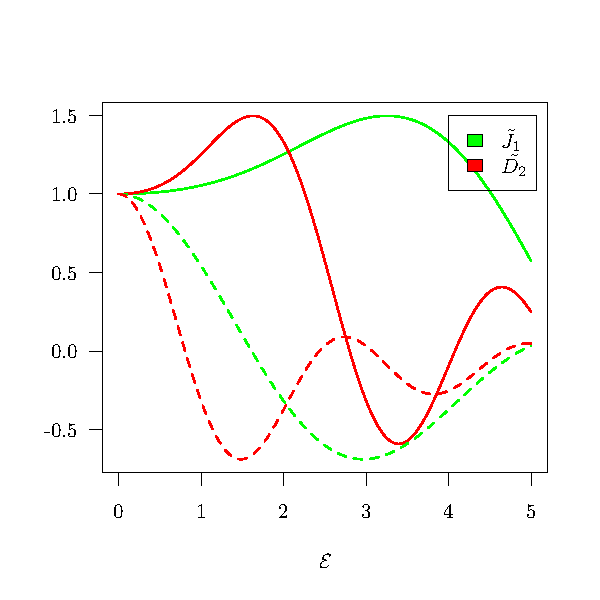
\includegraphics[width=\columnwidth]{../Figures/NNvsNNN.pdf}
\caption{For circularly polarized light we obtain $\tilde{J}_1 = \frac{J_{1,ij}'}{J_{1,ij}}$ and $\tilde{D}_{2} = \frac{D_{2,ij}'}{D_{2,ij}}$ as function of $\mathcal{E} = \frac{eaE_0}{\omega}$, where $e$ is the electron charge and $a$ is the lattice constant. The results are obtain for (units of $\hbar=t_1=1$) $t_2 = 0.1$, $\Delta = 0.5$, $\text{U} = 10$ and $\omega = 4, 14$. Solid lines are for $\omega = 4$ and dashed lines are for $\omega = 14$. For $\tilde{J}_1$, similar results are obtained by Mentink et Al. \cite{Mentink2015}.}
\label{fig2}
\vspace*{-6pt}
\end{figure}
A similar Hamiltonian including a NN exchange term and a NNN DMI term was first proposed by S. A. Owerre to model honeycome topological magnon insulators \cite{Owerre2016} \cite{Elyasi}. Additionally, experimental results regarding topological properties of spin waves in honeycomb ferromagnet Cr$I_3$ can only be understood by considering this Hamiltonian \cite{Chen2018}. This model is also relevant for the study of Spin Hall effects of Weyl magnons \cite{Zyuzin2018} \cite{Sekine2015}.

Now, a Hamiltonian with the form $\hat{H} = \sum_{\langle i,j \rangle} J_1 \bs{S}_i\bs{S}_j + \sum_{\langle \langle i,j \rangle \rangle} J_2\bs{S}_i\bs{S}_j$ is known as the $J_1$-$J_2$ Heisenberg model and in a 2D honeycomb lattice it exhibits N\'eel order for $J_2 < J_1 / 6$ and for $J_2 > J_1 / 6$ spin density waves (SDW) appear \cite{Mulder2010}. In the presence of DMI alone there will always be SDW in the plane perpendicular to $\bs{D}$ \cite{Uchida2006}. In Hamiltonian \ref{MKMHeff0} we expect SDW to appear in the ground state and the SDW wavevector will be determined by a function of the parameters of this model. We have shown that we can modulate these parameters thus providing a techique to manipulate the SDW in the ground state.

\begin{subsection}{Disorder}
It is possible to introduce the effect of disorder in the model \ref{MKMH} by adding random uncorrelated on-site energies:

\begin{align}
\label{DisorderedHubbardModel}
\hat{H}_0 &= - \sum_{\langle i,j \rangle, \sigma} t_1\hat{c}_{i \sigma}^\dagger \hat{c}_{j \sigma} -\sum_{\langle \langle i,j \rangle \rangle, \sigma}(t_2 - i\Delta\nu_{ij}\sigma^z_{\sigma, \sigma})\hat{c}_{i \sigma}^\dagger \hat{c}_{j \sigma} \n \\
	& + \sum_{i \sigma} \epsilon_i \hat{c}_{i \sigma}^\dagger \hat{c}_{i \sigma} +
	\text{U}\hat{D}
\end{align}

Where $\epsilon_i$ are uncorrelated random variables $\epsilon_i \in [-W,W]$. At half filling we can derive an effective Hamiltonian using the same procedure as before. The second order virtual hopping $i\sigma \rightarrow j\sigma \rightarrow i\sigma$ will give rise to an exchange spin interaction. In this case, however, the intermediate energy is $\text{U} + (\epsilon_j - \epsilon_i)$. Therefore the spin Hamiltonian will be:

\begin{align}
&\hat{H}_{\text{eff}}^{\text{Dis}} = \sum_{\langle i,j \rangle} J_{1,ij}\bs{S}_i\cdot\bs{S}_j +\n \\
&+ \sum_{\langle \langle i,j \rangle \rangle} \left\{ J_{2,ij}\bs{S}_i\cdot\bs{S}_j + \bs{D}_{2,ij}\cdot \bs{S}_i \times \bs{S}_j + \bs{S}_i \bs{\Gamma}_{ij} \bs{S}_j \right\}
\end{align}

With:

\begin{align*}
J_{1,ij}' &= \frac{2t_1^2\text{U}}{\text{U}^2-(\epsilon_j-\epsilon_i)^2} \\
J_{2,ij}' &= \frac{2t_2^2\text{U}}{\text{U}^2-(\epsilon_j-\epsilon_i)^2} \\
\bs{D}_{2,ij}' &= -\frac{4\nu_{ij} t_2 \Delta \text{U}}{\text{U}^2-(\epsilon_j-\epsilon_i)^2}\hat{e}_z \\
\bs{\Gamma}_{2,ij}' &= \frac{2\Delta^2\text{U}}{\text{U}^2-(\epsilon_j-\epsilon_i)^2}\text{diag}(-1,-1,1)
\end{align*}

Where in the second step we added the contributions of $\langle i,j \rangle$ and $\langle j,i \rangle$ and where $J_{ij} = \frac{2t^2\text{U}}{\text{U}^2-(\epsilon_j-\epsilon_i)^2}$. This model is relevant for studying many-body localization phenomena \cite{Protopopov2018}.
\end{subsection}

\end{section}

\section*{Acknowledgments}

%\begin{thebibliography}
\bibliography{../MT}
%\end{thebibliography}

\end{document}


